\setlength{\parskip}{1em}

\chapter{Zadání}

\textbf{Standardní zadání - webové stránky konferenčního systému}

Vaším úkolem bude vytvořit webové stránky konference.  Téma konference si můžete zvolit libovolné.\\
Uživateli systému budou autoři příspěvků (vkládají abstrakty a PDF dokumenty), recenzenti příspěvků (hodnotí příspěvky) a administrátoři (spravují uživatele, přiřazují příspěvky recenzentům a rozhodují o publikování příspěvků). Každý uživatel se bude do systému přihlašovat prostřednictvím uživatelského jména a hesla. Nepřihlášený uživatel vidí pouze publikované příspěvky.\\
Nový uživatel se bude moci zaregistrovat, čímž získá status autora.\\
Přihlášený autor vidí svoje příspěvky a stav, ve kterém se nacházejí (v recenzním řízení / přijat +hodnocení / odmítnut +hodnocení). Příspěvky může přidávat, editovat a volitelně i mazat.\\
Přihlášený recenzent vidí příspěvky, které mu byly přiděleny k recenzi, a může je hodnotit (alespoň 3 kritéria). Pokud příspěvek nebyl dosud schválen, tak své hodnocení může změnit.\\
Administrátor spravuje uživatele (určuje jejich role a může uživatele zablokovat či smazat), přiřazuje neschválené příspěvky recenzentům k ohodnocení (každý příspěvek bude recenzován minimálně třemi recenzenty) a na základě recenzí rozhoduje o přijetí nebo odmítnutí příspěvku. Přijaté příspěvky jsou automaticky publikovány ve veřejné části webu.\\
Databáze musí obsahovat alespoň 3 tabulky dostatečně naplněné daty pro předvedení funkčnosti aplikace.


%%%%%%%%%%%%%%%%%%%%%%%%%%%%%%%%%%%%%%%%%%%%%%%%%%%%%%%%%%%%%%%%%%%%%%%%%%%%%%%%%%%%%%%%%%%%%%%%%%%%

\chapter{Implementace}

Design webové aplikace je vytvořen pomocí frameworku \emph{Bootstrap}, \emph{CSS} (definován ve složce /css) a šablony \emph{Twig}.  Funkční část aplikace pak v \emph{PHP}.

Aplikace dodržuje MVC architekturu. Obsah jednotlivých stránek je ve složce /cont a /nav (navigace na stránkách). Funkční čast aplikace, tj. přihlašování, registrace, práce s články a práce s databází, v .php soborech ve složce /inc. Funkční část aplikace je znázorněna na diagramu na obrázku \ref{uml}. Zobrazení správného obsahu za pomoci Twigu zajišťuje soubor index.php v kořenovém adresáři. Přesměrování URL adresy na index.php je zajištěno souborem .htaccess.

Práce s databází je zajištěna pomocí rozhraní \emph{PDO}. Dotazy do databáze jsou skládány ve třídě /inc/db\_pdo.class.php. Tu pak implementují třídy /inc/db\_login.class.php a /inc/db\_articles.class.php, kde se tvoří konkrétní dotazy.

\begin{figure}[H]
	\centering
	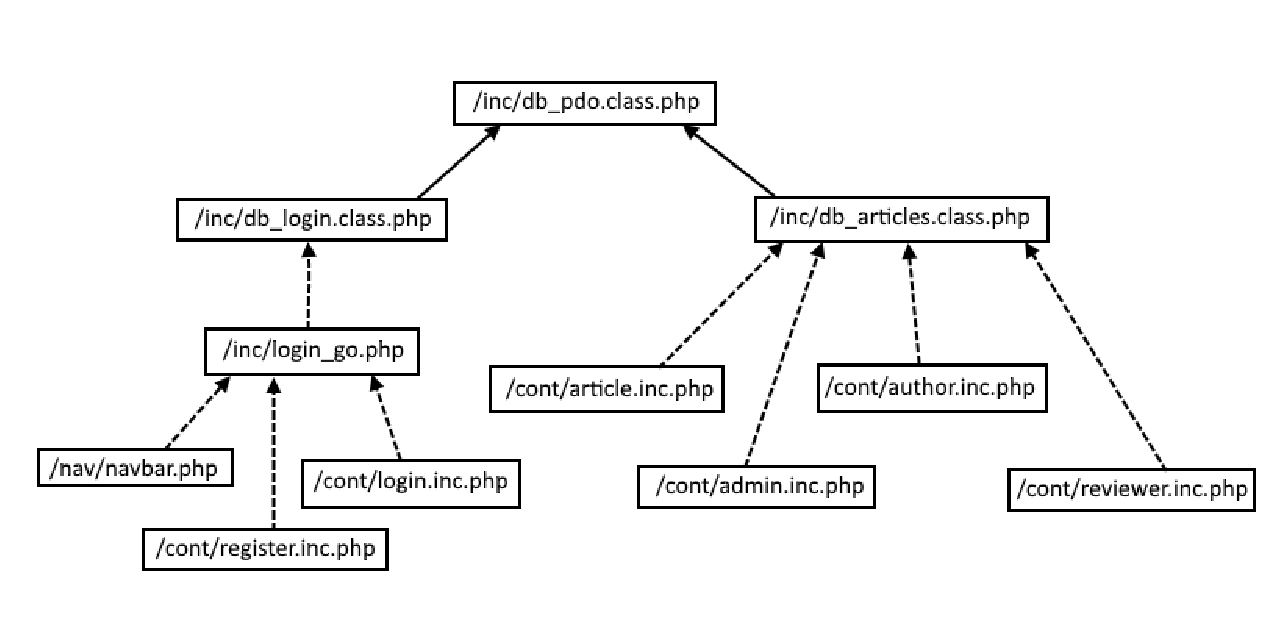
\includegraphics[width=1\textwidth]{img/UML.eps}
	\caption{Diagram funkční části aplikace}
  \label{uml}
\end{figure}


Na stránce \emph{Contact} je použitím javascriptu vložena Google mapa.

Nahrané soubory jsou uploadovány do složky /pdf na server. Lze nahrát pouze soubory formátu .pdf nebo .txt.


\section{Databáze}

Databáze má 4 tabulky (viz ERA diagram na obrázku \ref{eer}).

V tabulce \emph{users} je seznam registrovaných uživatelů. Tabulka \emph{rights} je seznam uživatelských práv. Tabulka \emph{articles} obsahuje všechny vložené články s ID uživatele, který je vložil, URL odkazu na soubor na serveru, ID na jednotlivá hodnocení od recenzentů (každý článek má tři hodnocení) a příznakem zda byl článek schválen. V tabulce \emph{score} jsou jednotlivá hodnocení přiřazená recenzentům (každé hodnocení má tři hodnoty).

\begin{figure}[H]
	\centering
	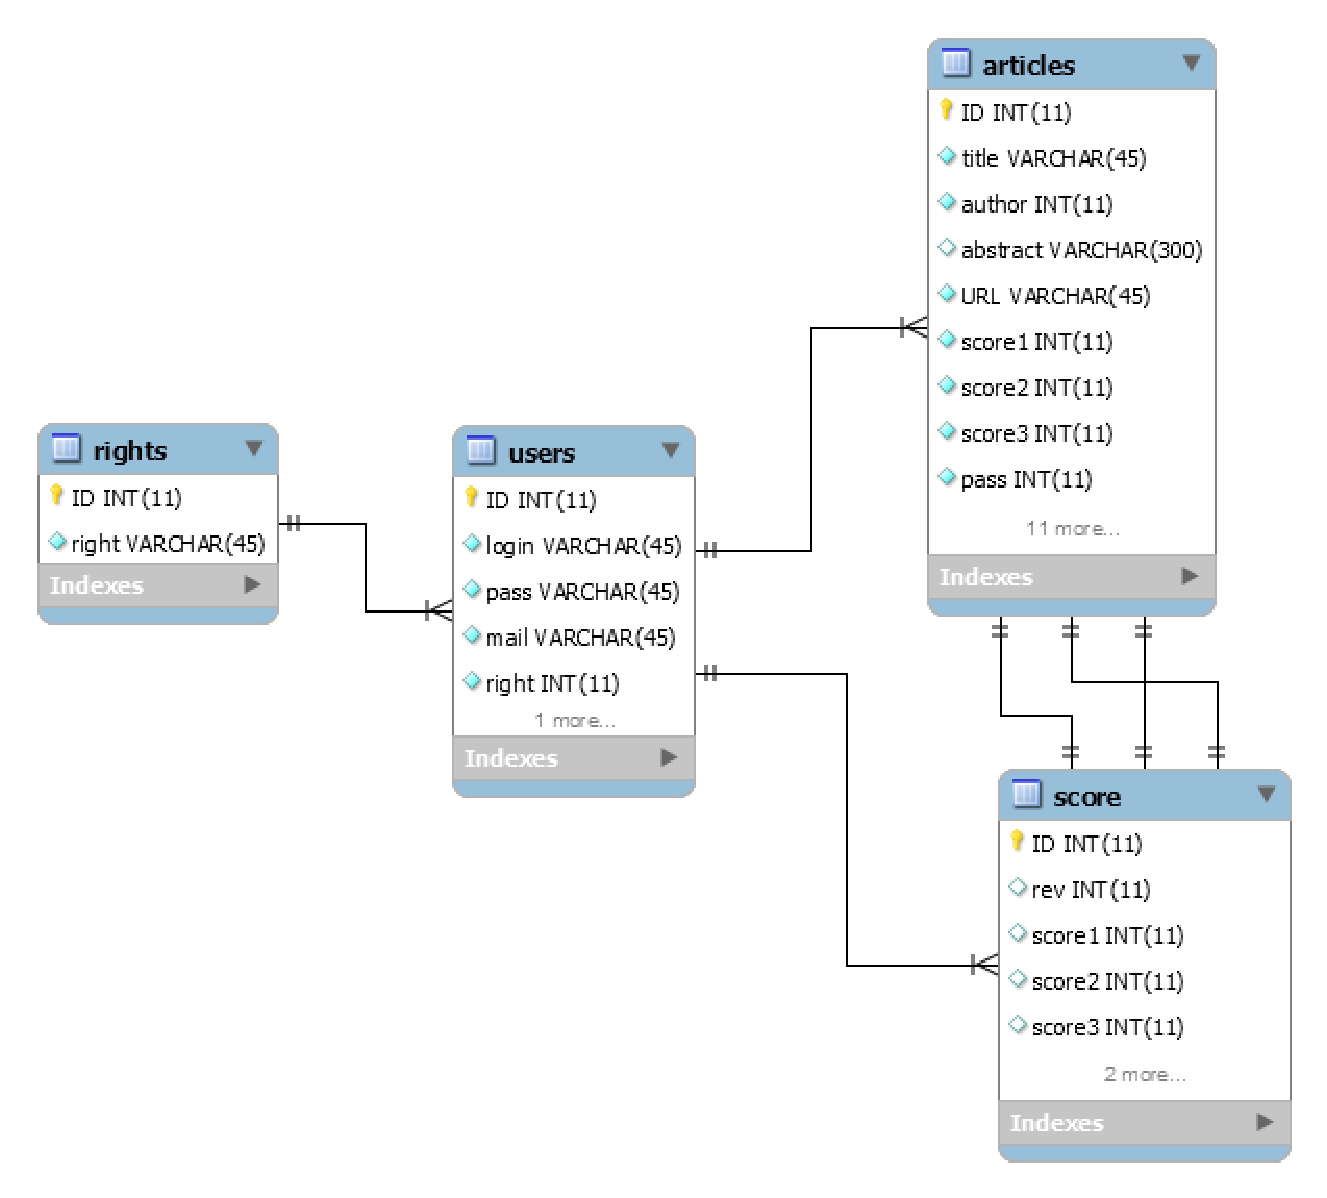
\includegraphics[width=1\textwidth]{img/web_sp_EER.eps}
	\caption{ERA diagram databáze}
  \label{eer}
\end{figure}


%%%%%%%%%%%%%%%%%%%%%%%%%%%%%%%%%%%%%%%%%%%%%%%%%%%%%%%%%%%%%%%%%%%%%%%%%%%%%%%%%%%%%%%%%%%%%%%%%%%%



\chapter{Závěr}

Zadání samostatné práce bylo splněno. Vytvořený návrh konferenčního systému je s menšími úpravami použitelný pro reálný konferenční systém.

Celý projekt je na GitHubu: \url{https://github.com/pivovard/web}.
